
\chapter{Function Merging}

In this section, we describe the proposed function-merging technique.
Contrary to the state-of-the-art, our technique is able to merge any two
functions.
If the two functions are equivalent, i.e., identical, then the two functions
can be completely merged into a single identical function.
However, if the two functions differ at any point, an extra parameter is
required, so that the caller is able to distinguish between the functions. 
The two functions can differ in any possible way, including their list of
parameters or return types.
If the lists of parameters are different, we can merge them so that we are able
to uniquely represent all parameters from both functions.
If the return types are different, we can use an aggregate type to return values
of both types or return just the non-void type if the other one is void.
%However, in our current implementation, the only restriction is that both
%functions must have equivalent return types or one of them must be \textit{void}.

\begin{figure}[h]
  \centering
  %\vspace{-1ex}
  \includegraphics[width=0.85\linewidth]{src/func-merging/figs/func-merge-overview.pdf}
  \caption{Overview of our function-merging technique.}
  \label{fig:func-merge-overview}
  %\vspace{-1ex}
\end{figure}

The proposed technique consists of three major steps, as depicted in
Figure~\ref{fig:func-merge-overview}.
First, we linearize each function, representing the CFG as a sequence of 
labels and instructions.
The second step consists in applying a sequence alignment algorithm, borrowed
from bioinformatics, which identifies regions of similarity between sequences.
The sequence alignment algorithm allows us to arrange two linearized functions
into segments that are equivalent between the two functions and segments where
they differ from one another.
The final step performs the code generation, actually merging the two functions
into a single function based on the aligned sequences.
Aligned segments with equivalent code are merged, avoiding redundancy, %redundant code,
and the remaining segments where the two functions differ have their code
guarded by a function identifier.
At this point, we also create a merged list of parameters where parameters of
the same type are shared between the functions, without necessarily keeping
their original order.
This new function can then be used to replace the original functions, as they
are semantically equivalent, given the appropriate function-identifier
parameter.

\subsection{Linearization}

The \textit{linearization}\footnote{Although linearization of CFGs
usually refers to a predicated representation, % resulting from an if-conversion,
in this paper, we refer to a simpler definition.}
of a function consits in specifying an ordering of the basic blocks based on a
traversal of the CFG and then producing a sequence of basic block labels and
instructions, similar to a textual representation of the function.
Although this operation is trivial, the specific ordering of the basic blocks
chosen can have an impact on the merging operation.

%For the linearization, we assume that every basic block has an entry label and
%a terminator instruction which refers explicitly to the successor basic blocks,
%if there are successors.
%This is true for most IRs, such as the LLVM IR, or can be easily adapted.

In our implementation, the linearization uses a reverse post-order~(RPO) of the
basic blocks, following a canonical ordering of the successors.
%, e.g., \textit{true} branches before \textit{false} ones.
%Figure~\ref{fig:branch-linearization} shows an example of the linearization 
%using the canonical RPO.
The RPO guarantees that the linearization starts with the entry basic block and
then proceeds favoring definitions before uses, except in the presence of loops.
Although the specifc ordering produced by the canonical linearization may not
be optimal, it is common practice for compilers to rely on prior
canonicalizations, e.g., 
canonical loops, canonical induction variables, canonical reassociation, etc.
For contrast, if, instead, we use an RPO linearization with a uniformly
randomized ordering of the successor basic blocks, the final code-size reduction
of the function-merging optimization can drop up to 10\% for individual
benchmarks.
Note that our decision for using the canonical RPO is purely pragmatic and
other orderings of the basic blocks could also be used, as long as it produces
a sequence of labels followed by instructions.

%\begin{figure}[h]
%  \centering
%  \includegraphics[width=0.6\linewidth]{figs/branch-linearization.pdf}
%  \caption{Linearization using a canonical reverse post-order.
%           The dashed arrows show where a randomized ordering could change the
%           linearization.}
%  \label{fig:branch-linearization}
%\end{figure}

\subsection{Sequence Alignment}

When merging two functions, the goal is to identify which pairs of instructions
and labels that can be merged and which ones need to be selected based on the
actual function being executed.
To avoid breaking the semantics of the original program, we also need to
maintain the same order of execution of the instructions for each one of
the functions.

To this end, after linearization, we reduce the problem of merging functions
to the problem of \textit{sequence alignment}. %~\cite{carrillo88,wang94}.
%After linearization, the problem of merging two functions can be reduced to the
%\textit{sequence alignment} problem~\cite{carrillo88,wang94}, which is itself
%closely related to finding the
%\textit{longest common subsequence}~\cite{hirschberg75,maier78}.
Sequence alignment is an important technique to many areas of science,
most notably in molecular biology~\cite{needleman70,smith81,carrillo88,wang94}
where, for example, it is used for identifying homologous subsequences of amino
acid in proteins.
Figure~\ref{fig:opcode-align} shows an example of the sequence alignment
between two linearized functions extracted from the \texttt{400.perlbench} benchmark
in SPEC CPU2006~\cite{spec}.

\begin{figure}[h]
  \centering
  \includegraphics[width=0.85\linewidth]{src/func-merging/figs/opcode-align.pdf}
  %\caption{An example of a sequence alignment between two real functions extracted from the \text{400.perlbench} benchmark.}
  \caption{The sequence alignment between two functions.}
  \label{fig:opcode-align}
\end{figure}

Formally, sequence alignment can be defined as follows:
For a given alphabet $\alpha$, a sequence $S$ of $k$ characters is a subset of
$\alpha^k$, i.e., $S = (a_1, \ldots a_k)$.
Let $S_1, \ldots, S_m$ be a set of sequences, possibly of different lengths but
all derived from the same alphabet $\alpha$, where
$S_i = (a_1^{(i)}, \ldots, a_{k_1}^{(i)})$, for all $i\in\{1,\ldots,m\}$.
%\begin{equation*}
%\begin{align*}
%S_1 = (a_1^{(1)}, \ldots, a_{k_1}^{(1)})\\
%\dots\\ 
%S_m = (a_1^{(m)}, \ldots, a_{k_m}^{(m)})
%\end{align*}
%\end{equation*}
Consider an extended alphabet that includes the \textit{blank} character ``$-$'',
i.e., $\beta = \alpha \cup \{-\}$.
An alignment of the $m$ sequences, $S_1, \ldots, S_m$, is another set of sequences,
$\bar{S}_1, \ldots, \bar{S}_m$, such that each sequence $\bar{S}_i$ is obtained
from $S_i$ by inserting blanks in positions where some of the other sequences
have non-blank and possibly equivalent characters, for a given equivalence relation.
All sequences $\bar{S}_i$ in the alignment set have the same length $l$, where
$\max\{k_1,\ldots,k_m\} \leq l \leq k_1 + \cdots + k_m$.
Moreover, $\forall i\in\{1,\ldots, m\}$, $\bar{S}_i = (b_1^{(i)},\ldots,b_l^{(i)})$,
there are increasing functions $v_i: \{1,\ldots,k_i\} \to \{1,\ldots,l\}$, such that:
\begin{itemize} %[noitemsep,topsep=0pt]
\item $b_{v_i(j)}^{(i)} = a_j^{(i)}$, for every $j \in \{1,\ldots,k_i\}$;
\item any position $j$ not mapped by the function $v_i$, i.e.,
for all $j \in \{1,\ldots,l\}\setminus \textrm{Im} v_i$,
then $b_j^{(i)}$ is a blank character.
\end{itemize}
Finally, for all $j\in\{1,\ldots,l\}$, there is at least one value of $i$ for
which $b_j^{(i)}$ is not a blank character.
%and for any pair of sequences that have a non-blank character at position $j$,
%these characters are equivalent.
Note that two aligned sequences may contain both non-blank and non-equivalent
characters at any given position, in which case it contains a mismatch.

Particularly for the function-merging, we are concerned with the alphabet
consisting of all possible typed instructions and labels.
Every linearized function represents a sequence derived from this alphabet.
We explain the equivalence relation used for this alphabet in the next section.

%We describe the equivalence relation between two predicated values in two
%separate cases, namely, the equivalence between instructions and the
%equivalence between labels.
%Labels are always considered equivalent.
%Two instructions are equivalent if their opcode are semantically equivalent,
%but not necessarily the same, and they both have types that can be bitcasted in
%a losslessly way from on to the other.
%This also includes making sure that there is no conflict regarding memory
%alignment when handling pointers.
%No additional restriction is imposed on the operands of the two instructions
%being compared for equivalence.
%Whenever two operands cannot be statically proved to represent the same value,
%a select instruction can be used to distinguish between the execution of two
%functions being merged.
%For function calls, the type equivalence requires that both instructions have
%identical function types, i.e., both called functions must have an identical
%return type and an identical list of parameter types. 

There is a vast literature on algorithms for performing sequence alignment,
especially in the context of molecular biology.
These algorithms range from optimal algorithms based on dynamic programming to
probabilistic models that does not guarantee
optimality~\cite{needleman70,smith81,carrillo88,hickey11}. 
In this paper, we use the Needleman-Wunsh algorithm~\cite{needleman70}.
This algorithm is based on dynamic programming and consists of two main steps.
First, it builds a \textit{similarity matrix}, based on a scoring scheme, which
assigns weights for matches, mismatches, and \textit{gaps} (blank characters).
Afterwards, a backward traversal is performed on the similarity matrix, in order
to reconstruct the final alignment by maximizing the total score.
We use a simple scoring scheme that rewards matches and penalizes mismatches and
gaps.

%\todo{Remove this paragraph.}
%When producing the final aligned sequence, there may be several possible optimal
%alignments.
%However, different aligned sequences can affect the code generation in different
%ways that may be both beneficial or undesirable. 
%For this reason, we prioritize alignments that tend to group the blank
%characters together, avoiding to frequently alternate between the two sequences
%during long segments of mismatches and gaps.
%For example, note that in Figure~\ref{fig:opcode-align}, the red blocks, for
%a particular sequence, tend to be grouped together.

\subsection{Equivalence Relation}

We describe the equivalence relation between values in two
separate cases, namely, the equivalence between instructions and the
equivalence between labels.

Labels can represent both normal basic blocks and landing blocks, which are used
in exception handling code.
Labels of normal basic blocks are always considered equivalent but
landing blocks must have exactly the same landingpad instructions.

Two instructions are equivalent if: $(1)$ their opcode are semantically
equivalent, but not necessarily the same; $(2)$ they both have equivalent types;
and $(3)$ they have pairwise operands with equivalent types.
Types are considered equivalent if they can be bitcasted in a losslessly way
from on to the other.
It is also important to make sure that there is no conflict regarding memory
alignment when handling pointers.
No additional restriction is imposed on the operands of the two instructions
being compared for equivalence.
Whenever two operands cannot be statically proved to represent the same value,
a select instruction is used to distinguish between the execution of two
functions being merged.
For function calls, the type equivalence requires that both instructions have
identical function types, i.e., both called functions must have an identical
return type and an identical list of parameter types. 

\subsubsection{Handling Exception Handling Code}

Most modern compilers implement the zero-cost Itanium ABI for exception
handling~\cite{dinechin00}, including GCC and LLVM, sometimes called the
\textit{landing-pad} model. In this section, we describe restrictions imposed
by exception handling code and their equivalence relation.

The invoke instruction co-operates tightly with its landing block, i.e., the
basic block pointed by the exception branch of an invoke instruction.
The landing block must landingpad instruction as its first non-$\phi$
instruction.
Given this restriction, two equivalent invoke instructions must also have
landing blocks with equivalent landingpad instructions.
This is easy to check since the landingpad instruction is always the first
instruction in a landing block. 

Landing blocks are responsible for handling all catch clauses of the
higher-level programming language covering the particular callsite.
All clauses are defined by the landingpad instruction, which encodes the list of
all exception and cleanup handlers.
Landingpad instructions are equivalent if they have the exactly same type and
also encode an identical lists of exception and cleanup handlers.
The type of equivalent landingpad instructions must be identical as its value
is crucial in deciding what action to take when the landing block is entered,
and corresponds to the return value of the personality function, which must also
be identical for the two functions being merged.

%The return value of the landingpad instruction is crucial in deciding what
%action to take when the landing block is entered, and corresponds to the return
%value of the personality function.

%In other words, when the unwinder executes the personality function (which
%is part of the language runtime), it stores its return value, and provides this return value in the result of the landingpad
%instruction. Since the personality function has access to the part of the unwind tables generated from the landingpad
%instruction, it can communicate information encoded in the unwind table to the landing block itself. In the libc++ runtime,
%the personality function returns a tuple consisting of a pointer to the exception object itself, and a “handler switch value”, an
%integer which corresponds to the index of a relevant “catch” clause of the landingpad instruction, or a special value (−1)
%when no catch clauses match but a cleanup needs to be performed.

%The LLVM IR generated for the landing block then checks the handler switch value computed by the personality function,
%and transfers control to a cleanup or handler block accordingly.

%Finally, if the selected handler is a cleanup handler, the
%exception propagation (stack unwinding) needs to be resumed after the cleanup is done. This is achieved by the resume
%instruction, which expects as a parameter the same value that was returned by the corresponding landingpad instruction
%which interrupted the exception propagation.
%Interestingly, there are no LLVM instructions for raising (throwing) exceptions. This is left entirely in the management
%of the language runtime, which needs to closely co-operate with the stack unwinding library anyway (the interface of the
%personality function is mandated by the stack unwinder).

